\chapter{Virtuelle Rekonstruktion}
\label{sec:minimal} 


(WICHTIG $\sigma$ zu $\tau$ umschreiben, da ja gesagt wird das S = I, sonst kommt Verwirrung auf)


Für den in dieser Arbeit benutzen Ansatz des Szenenrekonstruktionsalgorithmus, wird davon ausgegangen, dass die intrinsischen Kameraparameter bekannt sind. Der Grund dafür ist, dass in dieser Arbeit ein Ansatz entwickelt werden sollte, welcher die Möglichkeit von unterschiedlichen Auflösungen der Kameras mit einbeziehen sollte. Aus diesem Grund wurde ein Ansatz für die Szenenrekonstruktion entwickelt, welcher keine Rektifizierung der Bilder mit einschließt. \\

Im folgenden sollen die Funktionsweisen und Abläufe des entstandenen Szenenrekonstruktionsalgorithmus aufgezeigt werden. Hierzu wurde ein virtuelle Beispielszene gebaut mit einem 3D-Objekt und zwei simulierten zueinander rotierten und verschobenen Kameras. Das Objekt wird mathematisch auf die virtuellen Sensoren der beiden Kameras abgebildet. In Abblidung \ref{fig:ArbeitsProzessVirtuell} werden die einzelnen Schritte des Algorthmus nocheinmal schematisch kurz zusammengefasst. Die Schritte eins bis vier beschreiben den Aufbau der virtuellen Szene. In schritt drei der Einzelkalibrierung werden die intrinsischen Kameraparameter der beiden Kameras bestimmt. Ab hier setzt dann der Szenenrekonstruktionsalgorithmus an.

\begin{minipage}{\linewidth}
	\centering
	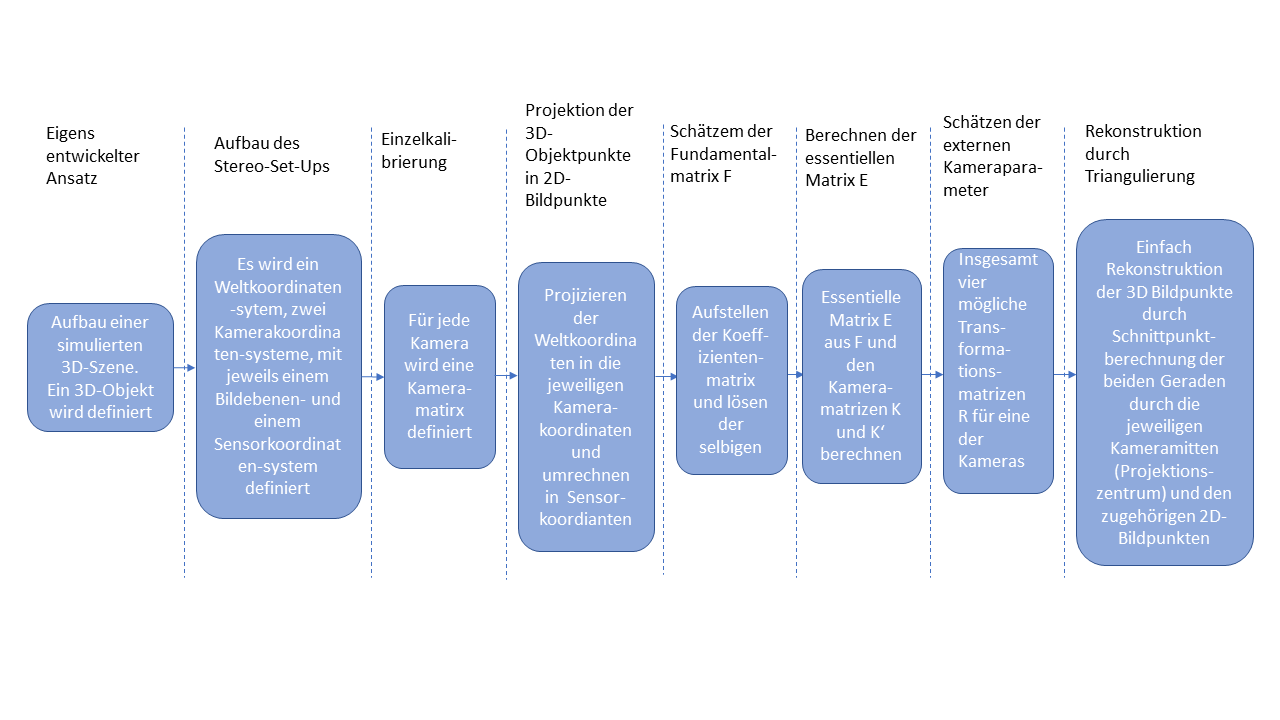
\includegraphics[width=1.\linewidth]{images/ArbeitsProzessMinimal.png}
	\captionof{figure}{Arbeitsprozesse der Stereoanalyse bei Verwendung von eigens erstellten synthetischen Bilddaten}
	\label{fig:ArbeitsProzessVirtuell}
\end{minipage}\\ \\

%
%Für die Entwicklung des Ansatzes für den Szenenrekonstruktionsalgorithmus sind  des Algorithmus sind 



\section{Erstellen eines virtuellen Stereoaufbaus}

Als 3D-Objekt wurde ein Quader, in ein Weltkoordinatensystem $(O,\delta)$ mit $\delta = (\hat{d_1},\hat{d_2},\hat{d_3})$ positioniert. Des Weiteren wurden zwei Kameras $(C,\beta)$ mit $\beta = (\hat{b_1},\hat{b_2},\hat{b_3})$ und $(C',\beta')$ mit $\beta' = (\hat{b'_1},\hat{b'_2},\hat{b'_3})$ in $(O,\delta)$ platziert. Das Weltkoordinatensystem $(O,\delta)$ und Das Kamerakoordinatensystem $(C,\beta)$ sind deckungsgleich. Im weiteren Verlauf werden die beiden Kameras jeweils mit $C$ oder $C'$ bezeichnet, um die Unterscheidung beider klar zu machen. $C'$ ist von $C$ entlang der x-Achse verschoben worden und um $45^\circ$ Richtung $C'$ rotiert. Die zwei Bildebenen $(I,\tau)$ mit $\tau = (\hat{t_1},\hat{t_2},\hat{t_3},I)$ und $(I,\tau)$ mit $\tau = (\hat{t_1},\hat{t_2},\hat{t_3},I)$ befinden sich vor $C$ und $C'$ in positiver z-Richtung. 
Anzumerken ist, dass für das virtuelle Beispiel angenommen wurde, dass Bildebenenkoordinatensystem und Sensorkoordinatensysetm gleich sind und deshalb mit der vereinfachten Kameramatrix $K_0$, siehe Kapitel \nameref{sec:CameraModels}.
Der schematische Aufbau der Szenen ist in den Abbildungen \ref{fig:aufbauMinimalTopDown}, \ref{fig:AbbildungenMinimal} und \ref{fig:KoordsystemeMinimal} dargestellt.


%Kamera eins $(C,\beta)$ ist Deckungsgleich mit $(O,\delta)$. Kamera zwei $(C',\beta')$ wurde von $C$ in positive $d_1$-Richtung, verschoben und um einen Winkel $\alpha$ zu $C$ um die eigene $b'_3$-Achse rotiert. Die verwendeten kartesischen Koordinatensysteme sind in diesem Minimalbeispiel alle rechtshändig orientiert. Die äußeren und inneren Kameraparameter wurden für den Aufbau der Szene festgelegt. Dies hat den positiven Effekt, dass somit die späteren Ergebnisse besser validiert werden können. In den Abbildung \ref{fig:aufbauMinimalTopDown} bis \ref{fig:KoordsystemeMinimal} wird der Aufbau noch einmal genauer veranschaulicht. \\

\begin{figure}[!htb]
	\minipage{0.52\textwidth}
	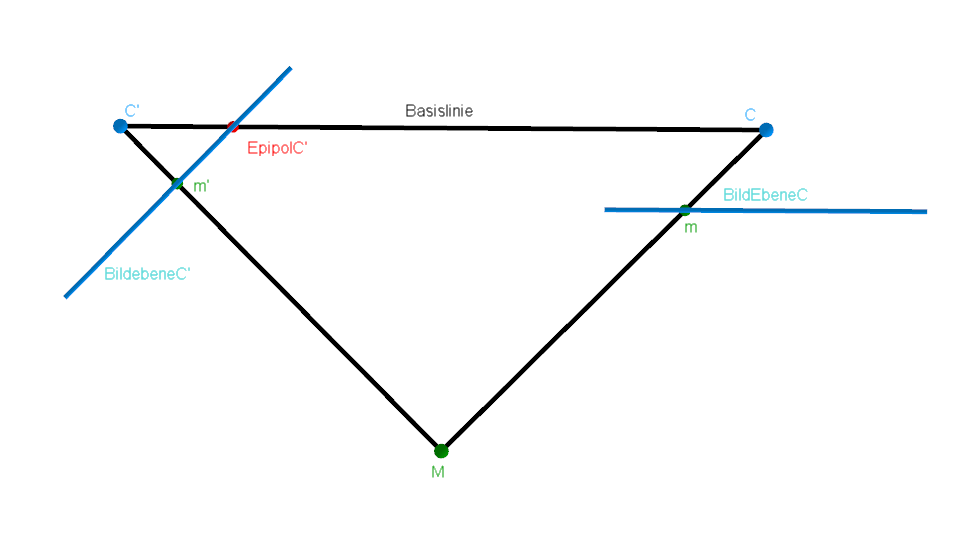
\includegraphics[width=\linewidth]{images/AufbauMinimalbeispiel.png}
	\caption{In der Abbildung ist der vereinfachte Stereoaufbau in einer Top-Down-Ansicht zu sehen}
	\label{fig:aufbauMinimalTopDown}
	\endminipage\hfill
	\minipage{0.42\textwidth}
	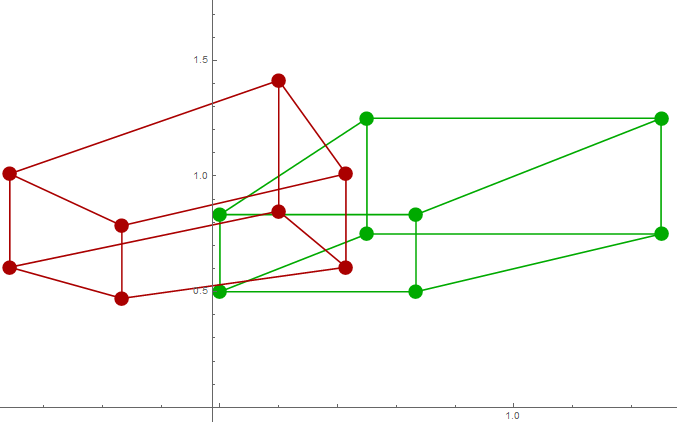
\includegraphics[width=\linewidth]{images/QuadrateMinimalBeispiel.png}
	\caption{In Grün ist die Abbildung des Quaders auf der Bildebenen $I$ von $C$ und in rot ist die Abbildung des Quaders auf der Bildebenen $I'$ von $C'$ zu sehen}
	\label{fig:AbbildungenMinimal}
	\endminipage\hfill
\end{figure}

\begin{minipage}{\linewidth}
	\centering
	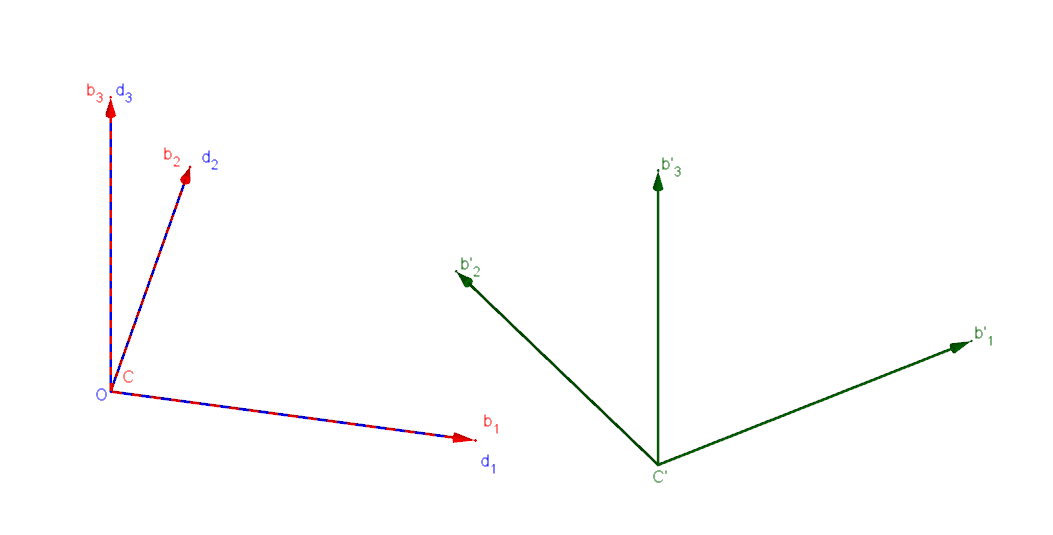
\includegraphics[width=.52\linewidth]{images/KS_Minimalbeispiel.png}
	\captionof{figure}{\textcolor{red}{Achsen falsch!!!}In Blau und Rot sind jeweils das Welt- und Kamerakoordinatensystem von Kamera eins zu sehen . In grün ist das gedrehte Koordiantensystem von Kamera 2 zu sehen.}
	\label{fig:KoordsystemeMinimal}
\end{minipage}\\ \\

%
%Für die Stereokamerakalibrierung wird $C'$ relativ zur zu $C$ um einen Vektor \ensuremath{\vec{V'}} verschoben und anschließend um einen Winkel \ensuremath{\alpha} um die $b'_3$ Achse gedreht. Für die Rotation um \ensuremath{b'_3} wird eine Drehmatrix $D'$ aufgestellt.

Zunächst werden die extrinsischen Kameraparameter von $C$ und $C'$ definiert. $C$ ist gegenüber $O$ weder rotiert noch verschoben, $C'$ dagegen ist entlang $\hat{d_1}$ verschoben und um $\hat{b_2}$ rotiert. Somit ergibt sich für $R=[D|V]$ von $C$:

%Dabei gehen wir davon aus, dass $C$ weder rotiert noch verschoben ist, während $C'$ verschoben und rotiert ist.(Hier eher wieder allgemein bleiben C gegenüber O keine verönderung C' schon)


\begin{gather}
	V=\begin{pmatrix}
		0\\0\\0
	\end{pmatrix}\\
	R = [I|V]\\
	R = \begin{bmatrix}
		1&&0&&0&&v_1\\
		0&&1&&0&&v_2\\
		0&&0&&1&&v_3
	\end{bmatrix}
\end{gather} 


%Die entstandene Matrix \ensuremath{R'} beschreibt die Transformation $C'$ und somit auch die Transformation von Punkten des Koordinatensystems $(C,\beta)$ in $(C',\beta')$. Da $(C,\beta) = (O,\delta)$ ist, beinhaltet die Transformationsmatrix $R$ für $C$ weder eine Translation noch eine Rotation.

Und für $R'=[D'|V']$ von $C'$ gilt:

\begin{gather}		
		R'=D'^T\cdot [I|V]\\
	D'= 
	\begin{pmatrix}
		\cos(\alpha)&0&\sin(\alpha)\\
		0&1&0\\
		-\sin(\alpha)&0&\cos(\alpha)
	\end{pmatrix}\\
	\vec{V'}= 
	\begin{pmatrix}
		1&0&0&-v'_1\\
		0&1&0&-v'_2\\
		0&0&1&-v'_3			
	\end{pmatrix}\\
	R'=		\begin{pmatrix}
		\cos(\alpha)&0&-\sin(\alpha)\\
		0&1&0\\
		\sin(\alpha)&0&\cos(\alpha)
	\end{pmatrix} 
	\cdot
	\begin{pmatrix}
		1&0&0&-v'_1\\
		0&1&0&-v'_2\\
		0&0&1&-v'_3			
	\end{pmatrix}\\
	R'=
	\begin{pmatrix}
		\cos(\alpha)&0&-\sin(\alpha)&-v'_1\cos(\alpha)+v'_3\sin(\alpha)\\
		0&1&0&-v'_2\\
		\sin(\alpha)&0&\cos(\alpha)&-v'_1\sin(\alpha)-v'_3\cos(\alpha)\\
	\end{pmatrix}
\end{gather}\\

%\section{Berechnung der Projetkionsmatritzen }

Die Eckpunkte des Quaders $A_\delta,B_\delta,C_\delta,D_\delta,A'_\delta,B'_\delta,C'_\delta,D'_\delta$ sind bekannt. Neben den Eckpunkten des Quaders wird noch ein neunter Punkt $E_\delta$ außerhalb des Quaders platziert und zwar so, dass es zu keinen linearen Abhängigkeiten zwischen $E_\delta$ und den anderen Punkten kommt. So kann vermieden werden, dass die später aufgestellt Koeffizientenmatrix, zum berechnen der Fundamentalmatrix, einen Rang kleiner als acht bekommt und somit zwei linear unabhängige Lösungen ausgibt\cite{HZ}. 

%Im Unterkapitel \nameref{sec:MinimalFun} wird nochmal genauer drauf eingegangen, was das für $F$ bedeutet. Fürs erste wird festgelegt, dass insgesamt neun Punkte sich in der Szene befinden.

 Um diese Punkte auf die Bildebenen $(I,\tau)$ und $(I',\tau)$ zu projizieren, müssen neben den Transformationsmatrizen $R$ und $R'$ noch die Kameramatrizen $K$ und $K'$ festgelget werden.


\begin{gather}		
K =
\begin{bmatrix}
\zeta_{C}&0&0&0\\
0&\zeta_{C}&0&0\\
0&0&\zeta_{C}&0\\
%0&0&1&0
\end{bmatrix}\\
K' =
\begin{bmatrix}
\zeta_{C'}&0&0&0\\
0&\zeta_{C'}&0&0\\
0&0&\zeta_{C'}&0\\
%0&0&1&0
\end{bmatrix}
\end{gather}

Sind $R,R',K$ und $K'$ bekannt, können die Projektionsmatrizen $P$ und $P'$ gebildet werden. 


\begin{gather}
%R=
%\begin{bmatrix}
%1&&0&&0&&v_1\\
%0&&1&&0&&v_2\\
%0&&0&&1&&v_3
%\end{bmatrix}\\
P = K\cdot R \\
P =
\begin{bmatrix}
\zeta_{C}&0&0&0\\
0&\zeta_{C}&0&0\\
0&0&\zeta_{C}&0\\
%0&0&1&0
\end{bmatrix}\\
P' = K' \cdot R'\\
P' =
\begin{bmatrix}
\zeta_{C'} \cos(\alpha)&0&\zeta_{C'} \sin(\alpha)&-\zeta_{C'} (v'_1\cos(\alpha)+v'_3\sin(\alpha) )&0\\
0&1&0&\zeta_{C'}-v'_2&0\\
\zeta_{C'}\sin(\alpha)&0&\zeta_{C'}\cos(\alpha)&-\zeta_{C'}(v'_1\sin(\alpha)+v'_3\cos(\alpha))\\
%0&0&0&0&1
\end{bmatrix}
\end{gather}



%\section{Transformation der Objektpunkte von Weltkoordinaten in Kamerakoordinaten}

Die 3D-Punkte $A_\delta,B_\delta,C_\delta,D_\delta,A'_\delta,B'_\delta,C'_\delta,D'_\delta, E_\delta$, werden mit den Projektionsmatrizen \ensuremath{P} und \ensuremath{P2} auf die Bildebenen $I$ und $I'$ projizierten. Ein Beispiel für die entstehende Abbildung ist in Abbildung \ref{fig:AbbildungenMinimal} zu sehen. Da festgelegt wurde dass Sensorkoordinatensystem und Bildebenenkoordinatensystem Deckungsgleich sind, ist somit das Objekt auf den Bildebenen der virtuellen Kameras projiziert und es kann der Szenenrekonstruktionsalgorithmus beginnen.



\section{Bildanalyse}
\label{sec:MinimalFun}

Der Szenenrekonstruktionsalgorithmus für die virtuelle Rekonstruktion ist in drei Abschnitte unterteilt. Zuerst wird aus den Punktekorrespondenzen die Fundamentalmatrix und die essentielle Matrix berechnet geschätzt. Aus der essentiellen Matrix werden die extrinsischen Kameraparameter extrahiert um so im letzten Schritt durch Triangulation die Szenenpunkte zu rekonstrukieren. 

\subsection{Bestimmung der Abbildungsvorschriften}

Zu aller erst wird die Fundamentalmatrix $F$ aus den korrespondiernden Punkten bestimmt. Die korrespondierenden Punkte sind die jeweiligen Abbildungen der entsprechenden Eckpunkte. Anhand des in Kapitel \ref{sec:HFE} beschriebenen 8-Point-Algorithms, wird $F$ bestimmt. Über F wird die essentielle Matrix $E$ ermittelt. Vorraussetzung dafür ist, das die intrinsischen Kameraparameter bekannt sind.\\


%Um den Schnittpunkt der Gerade $B$ mit der Ebene $I$ zu berechnen, wird die Gerade $B$ in die Ebenengleichung eingesetzt und es wird ein Wert für $t$ ermittelt. 
%\begin{gather}
%\vec{n_0}\cdot \vec{x} - \vec{n_0}\cdot \vec{a}
%\end{gather}
%
%Danach wird die Geradengleichung \ensuremath{BaseLine} in die Ebenengleichung \ensuremath{ImagePlane} eingesetzt und es wird ein Wert für \ensuremath{t} ermittelt. Der berechnete Wert für $t$ wird dann wiederum in $G$ eingesetzt und das Ergebnis ist der Epipol \ensuremath{e'_\beta}. Dieser kann dann wieder über bereits bekannte Transformationen in die Sensorkoordinaten von $(S',\sigma)$ bezüglich $C'$ überfürht werden.
%
%\begin{gather}
%e'_\sigma=P'.e'_\beta
%\end{gather}
%
%Für die Epipolarlinien $l'_{\sigma'}$ durch $e'_{\sigma'}$, müssen einfach Geradengleichungen eines Sensorpunktes, beispielsweise $A_{\sigma'}$, durch $e_{\sigma'}'$ aufgestellt werden. Die entstandenen Linie ist dann die Epipolarlinie zum Punkt $A_{\sigma'}$ und gleichzeitig die korrespondierende Epipoloarlinie zum Sensorpunkt $A_\sigma$ von $I$ von $C$.
%
%\begin{gather}
%	g:= A_{\sigma'} +t \cdot (A_{\sigma'}-e'_{\sigma'})
%\end{gather}

%\subsection{Essentielle Matrix}


Für die Rekonstruktion der externen Kameraparameter, gibt es verschiedene Ansätze \cite{HZ}. Es ist zum einen Möglich, ohne Vorwissen der Kameramatrizen oder Transformationsmatrizen, aus der Fundamentalmatrix über den sogenannten \textit{Stratified approach} die komplette Projektionsmatrix $P$ und $P'$ zu ermitteln, jedoch ohne weitere Informationen über die 3S-Szene nur bis zu einem Projektiven Vieldeutigkeit\cite{HZ}. \\

Da in dieser Arbeit davon ausgegangen wird, dass die Kameras zuvor einzeln Kalibriert wurden und die intrinsischen Kameraparameter bereits bekannt sind, wird für die Rekonstruktion der externen Kameraparameter ein Ansatz verfolgt, in welchen die essentielle Matrix zum Einsatz kommt. Die essentielle Matrix ist eine Spezialform der Fundamentalmatrix und beschreibt den \textit{epipolar constraint}, zwischen den normierten Bildebenenkoordinaten\cite{HZ,Elements,ZZGXr,Zhang2014,Ferid}. 

(vllt $\tau$ schreiben? keine verwirrung mit anfang, macht schlussendlich bis auf die werte keien unterschied)
\begin{gather}
\hat{m}'^T_{\sigma'}.E.\hat{m}_\sigma = 0 
\end{gather}\\ 

Sind $F$ und Kameramatrizen $K$ und $K'$ bekannt, kann die essentielle Matrix wie in Kapitel \ref{sec:epipolar} gezeigt aus $F$ bestimmt werden.

%Ist die Fundamentalmatrix $F$ bereits ermittelt worden und die Kameramatrizen $K$ und $K'$ bekannt, kann die essentielle Matrix wie im Kapitel \nameref{sec:epipolar} aus $F$ berechnet werden. 
Die essentielle Matrix ist eine Fundamentalmatrix, welche zu einem paar normierter Projektionsmatrizen $P$ mit $P = [I|0]$ und $P'$ mit $P'= [R'|V']$ korrespondierend ist\cite{HZ,Zhang2014,ZZGXr,Ferid}. Um eine Projektionsmatrix $P'=K'[R'|V']$ auf die normierte Form zu bringen, müssen die intrinsischen Parameter für $K'$ bekannt sein. 

\begin{gather}
	m'_{\sigma} = P' \cdot M_\delta\\
	m'_{\sigma} = K'[R'|V'] \cdot M_\delta\;\; | \cdot K'^{-1}\\
	K'^{-1} \cdot m'_{\sigma} = K'^{-1} \cdot K'[R'|V'] \cdot M_\delta\\
	\hat{m}'_{\sigma} = [R'|V'] M_\delta
\end{gather}

$M_\delta$ ist der ein Objektpunkt im 3D-Raum, welcher mit $P'$ zum Bildebenenpunkt $m'_{\tau'}$ abgebildet wird. 

Nach der Normierung, wird $\hat{m}'_{\sigma}$ als normaierte Koordinate bezeichnet und die entstandene Projektionsmatrix $P' = [R'|V']$ als normierte Projektionsmatrix\cite{HZ,Ferid}.  Um $E$ aus $F$ zu gewinnen, werden die Kameramatrizen $K$ und $K'$ mit $F$ multipliziert. Zu Erinnerung im Kapitel \nameref{sec:epipolar} wurde genau diese Beziehung zwischen $E$ und $F$ hergestellt.


\begin{gather}
E = K'^TFK
\end{gather}

Das Ergebnis alle seine Vielfachen, sind mögliche Lösungen für die essentielle Matrix. Wie die Fundamentalmatrix muss auch die essentielle Matrix einen Rang von 2 haben. Des Weiteren darf eine 3x3-Matrix nur dann als essentielle Matrix bezeichnet werden, wenn die Singulärwerte, bestimmte Merkmale aufweisen. So müssen zwei der drei Singulärwerte gleich und die dritte null sein\cite{HZ}. Des Weiteren muss für die Determintante gelten, dass $det(E) = 0$ ist und die Quadratwurzel der Eigenwerte müssen wieder die Singulärwerte ergeben. Die essentielle Matrix kann, wie die Fundamentalmatrix auch, über den \textit{8-Point-Algorithm} ermittelt werden. Jedoch müssen auch hier die intrinsischen Kameraparameter $K$ und $K'$ bekannt sein, außerdem müssen die Koordinaten in normierte Bildebenkoordinatenumgerechnet werden.\cite{HZ,Ferid}.


\subsection{Bestimmung der externen Kameraparameter}


Mit der essentiellen Matrix ist es möglich die Transformationsmatrix $R'$ zu ermitteln. Es wird davon ausgegangen, dass für $R$ von $C$ gilt $R = [I|0]$. Die aus $E$ ermittelte Matrix $R'$ beschreibt dann die Transformation von $C'$ relativ zu $C$\cite{HZ,Ferid}. Um die externen Kameraparameter zu bestimmen, wird zunächst die essentielle Matrix \ensuremath{E} mit Hilfe der Singulärwertszerlegung in drei Matrizen zerlegt. 

\begin{gather}
E = U\Sigma V^T
\end{gather}

Die Singulärwerte befinden sich in der mittleren Matrix $\Sigma = diag(\sigma_1,\sigma_2,\sigma_3)$ wieder. Damit die Matrix $E$ sich essentielle Matrix nennen darf, muss für zwei der Diagonaleinträge für die Singulärwerte gelten das $\sigma_1 = \sigma_2$ und für $\sigma_3$ muss dann dementsprechend gelten, dass $\sigma_3=0$ anderes wäre sie keine singuläre Matrix.\\ 

%Sollten die Singulärwerte diesen Bedingungen nicht entsprechen, so wird ein so genannter \textit{singularity-constraint}, der Form $\Sigma = diag(\frac{\sigma_1+ \sigma_2}{2},\frac{\sigma_1+\sigma_2}{2},0)$, erzwungen\cite{HZ}. Im Minimalbeispiel kommt es auf Grund der eigens erstellten Bildpunkte zu keinen Bildfehlern, wie im Realbeispielen. Deswegen ist der \textit{singularity-constraint} nicht notwendig, da die Bedingungen für $E$ erfüllt sind.\\

%Ein wichtiges Detail, was sich später auch auf die vier möglichen Ergebnisse für $P$ auswirkt, ist noch zu beachten. Zum einen sollte einem bewusst sein, dass d

Die Zerlegung der essentiellen Matrix in $USV^T$ muss nicht zwingend eine eindeutige Lösung hervorbringen. Für $E$ muss gelten, dass $\text{det}(E) = 0$ ist. Es wird also vorausgesetzt, dass die Determinante der aus der $SVD$ gewonnen Matrizen $UV^T = 1$ ist. Angenommen aus der $SVD$ von $E$ ergibt sich für die Determinanten von $UV^T = -1$, so können die Determinanten der Matrizen $U$ und $V$ getrennt voneinander bestimmt werden. Sollte $\text{det}(U)=-1$ oder $\text{det}(V)=-1$ oder beides zusammen der Fall sein, so kann die jeweilige Matrix einfach mit $-1$ multipliziert werden.(Hab ich aus einer nicht zitierbaren quelle... wurde mal besprochen und eingebaut im code...)\\

$E$ setzt sich zusammen aus einer Rotationsmatrize $D$ und einer schiefsymmetrischen Matrix $S$\cite{HZ}. 

\begin{gather}
E=[v]_xR\\
S =[v]_x\\
E=SR
\end{gather}

Zur Schätzung von $S$ und $D$ werden des Weiteren die schiefsymmetrische Matrix \ensuremath{W} und die Blockdiagonale Matrix \ensuremath{Z} eigeführt\cite{HZ}. Mit diesen Matrizen lassen sich die gesuchten $D$ und $S$ für $C'$ rekonstruieren, jedoch nur bis zu einer gewissen Skaleninvarianz\cite{HZ,Ferid}.


\begin{gather}
W = \begin{pmatrix}
0&-1&0\\
1&0&0\\
0&0&1
\end{pmatrix} \;\;\;
Z=
\begin{pmatrix}
0&1&0\\
-1&0&0\\
0&0&0
\end{pmatrix}
\end{gather}

Mit dem Ergebnis der $SVD$ von \ensuremath{E} lassen sich nun jeweils zwei mögliche Lösungen für $S$ und $D$ aufstellen.


\begin{gather}
S_1 = -UZU^T \;\;\;\; D_1 = UW^TV^T\\
S_2 = UZU^T \;\;\;\; D_2 = UWV^T
\end{gather}\\


Um sicher zu gehen, dass es sich bei \ensuremath{D_1} und \ensuremath{D_2} auch um gültige Rotationsmatrizen handelt, kann eine Probe durchgeführt werden. Zum einen muss \ensuremath{D\cdot D^T=I_{3x3}} sein. \ensuremath{I_{3x3}} steht für die 3x3-Einheitsmatrix.  $S_1$ und $S_2$ sind jeweils schiefsymmetrische Matrizen, welche die Information für den noch gesuchten Vektor $\vec{v}$ beherbergt\cite{HZ}. 

\begin{gather}
St = [v]_\times \cdot v = v \times v
\end{gather} 

Um $v$ zu ermitteln muss lediglich der Kern von $S_1$ und $S_2$ gefunden werden. Die jeweilgen Ergebnisse für $v_1$ und $v_2$ sind bis auf ihre Vorzeichen die selben. Jedoch lässt sich hier $\vec{x}$ nur bis auf eine Skaleninvarianz genau bestimmen.(Grund nochmal finden... vergessen wo der stand... und was er war...). Die externen Kamerparameter lassen sich wie gesagt nur bis zu einem Skalierungsfaktor genau bestimmen\cite{HZ,Ferid}. Wie die Skaleninvarianz im virutellen Beispiel gelöst wurde, wird im nachfolgenden Abschnitt der Szenenrekonstruktion durch Triangulierung noch erklärt. \\

Letztendlich können, für die Rekonstruktion der externen Kameraparameter vier mögliche Lösungen für $R$ gefunden werden.\cite{HZ,Ferid}. $\lambda v$ heißt dabei, dass sowohl $v$ also auch alle Vielfache von $v$, Lösungen sein können, was durch die Skaleninvarianz der Resultate bedingt ist\cite{HZ,Ferid}. 

\begin{gather}
R = [UWV^T|+\lambda v] \;\;\; \textit{oder} \;\;\;[UW^TV^T|+\lambda v]\\
\textit{oder}\;\;\; [UWV^T|-\lambda v] \;\;\; \textit{oder} \;\;\;[UW^TV^T|-\lambda v]
\end{gather}

\begin{figure}[!htb]
	\minipage{0.52\textwidth}
	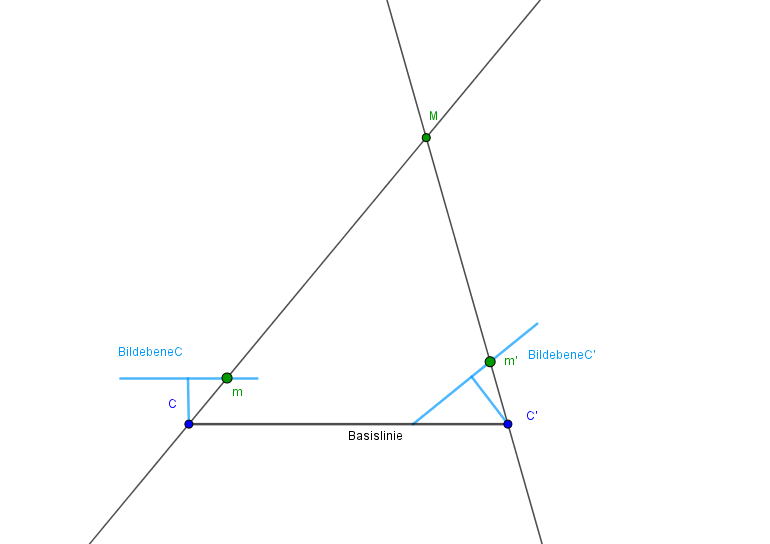
\includegraphics[width=\linewidth]{images/P_Solution_one.png}
	%	\caption{A really Awesome Image}
	\label{fig:awesome_image1}
	\endminipage\hfill
	\minipage{0.52\textwidth}
	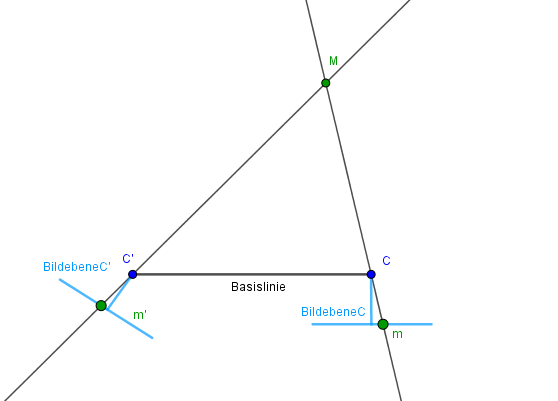
\includegraphics[width=\linewidth]{images/P_Solution_two.png}
	%	\caption{A really Awesome Image}
	\label{fig:awesome_image2}
	\endminipage\hfill
\end{figure}
\begin{figure}[!htb]
	\minipage{0.52\textwidth}
	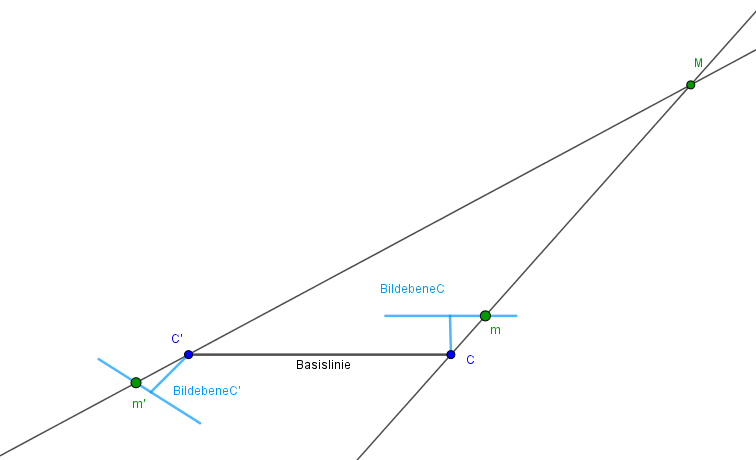
\includegraphics[width=\linewidth]{images/P_Solution_three.png}
	%	\caption{A really Awesome Image}
	\label{fig:awesome_image1}
	\endminipage\hfill
	\minipage{0.52\textwidth}
	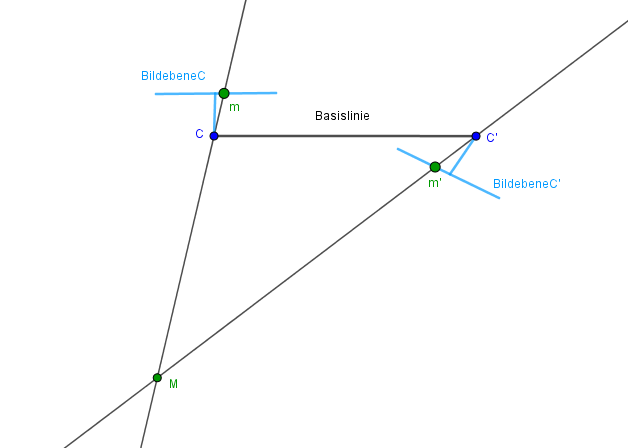
\includegraphics[width=\linewidth]{images/P_Solution_four.png}
	%	\caption{A really Awesome Image}
	\label{fig:awesome_image2}
	\endminipage\hfill
	\caption{Die Abbildung zeigt die vier möglichen Lösungen für $R$. }
\end{figure}
\pagebreak

(Noch einen Ansatz einbauen wie man die richtige Lösung algorithmisch auswertet? Im implementierte Algorithmus der arbeit wurden die Vier Lösungen jeweils rekonstruiert und alle ergebnisse ausgegeben.)

\subsection{Szenenrekonstruktion durch Triangulation}


Unter Triangulierung versteht man das Rekonstruieren der 3D-Szenenpunkte durch Schnittpunktberechnung derjenigen Geraden, welche durch die jeweiligen Projektionszentren der Kameras und deren korrespondierenden Bildpunkte auf deren Bildebenen gehen, so dass sich ein Dreick bildet.\\


\begin{minipage}{\linewidth}
	\centering
	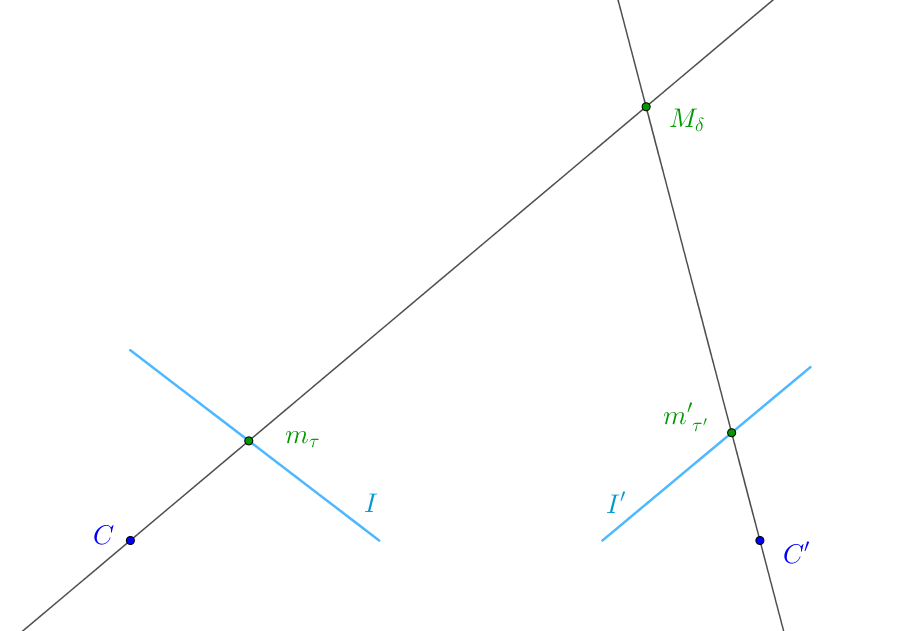
\includegraphics[width=0.8\linewidth]{images/optimaleTriangulierung.png}
	\captionof{figure}{Optimale Triangulierung: Beide Geraden Treffen sich in einem Punkt im 3D-Raum} 
\end{minipage}\\ \\


Da das Minimalbeispiel mit reinen Daten arbeitet, ist damit garantiert, dass die Linien sich in einem Schnittpunkt treffen. Anders hingegen wäre es in einem realen Beispiel mit korrespondierenden Punkten, welche Beispielsweise über einen \textit{SURF}- Algorithmus detektiert wurden\cite{Mandun}. In Realbildern, können Bildfehler wie beispielsweise Rauschen nicht vermieden werden, des Weiteren können korrespondierende Punkte nicht immer exakt auf den Pixel genau bestimmt werden. Diese Fehler führen dazu, dass wenn ein Schnittpunkt der Geraden durch die vermeintlichen korresponiderenden Punkte nicht gefunden werden kann, da die Geraden sich sehr wahrscheinlich nicht in einem Punkt treffen werden\cite{Mandun,HZ}. 


\begin{minipage}{\linewidth}
	\centering
	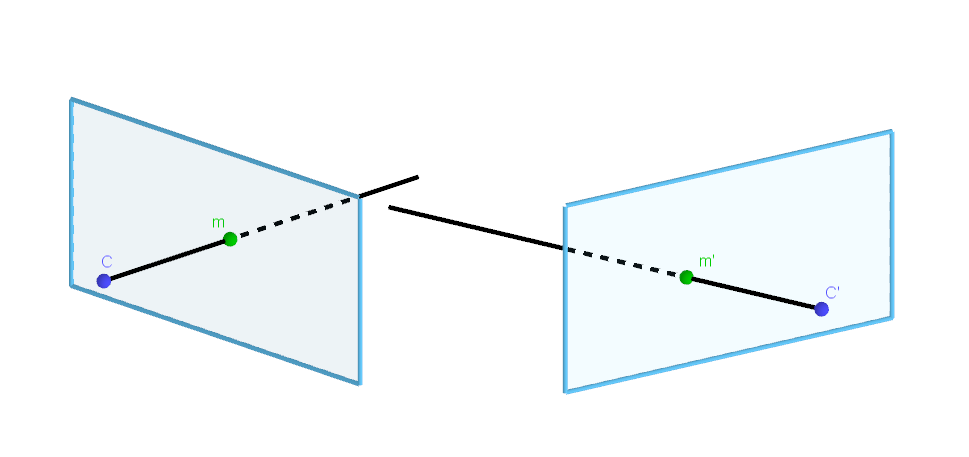
\includegraphics[width=0.8\linewidth]{images/problemTriangulation.png}
	\captionof{figure}{Durch Ungenauigkeiten in der korrespondierenden Punkte, verfehlen sich die Linien und es kommt zu keinem Schnittpunkt} 
\end{minipage}\\ 

Für diese Fälle gibt es mehrere Näherungsverfahren, wovon eines, im Kapitel \nameref{sec:sampson}, im Realbeispiel eingeführt wird\cite{HZ}. In diesem Minimalbeispiel tritt der optimale Fall ein. Das bedeutet, dass ein zu Bildpunkt $m$ korrespondierender Bildpunkt $m'$ auf der zu $m$ korrespondierenden Epipolarlinie $l'$ liegt und somit garantiert ist, dass sich die Geraden $\overline{mM}$ und $\overline{m'M}$ auf jedenfall in einem gemeinsamen Punkt schneiden. Um den Schnittpunkt beider Geraden zu berechnen, werden zum einen die Bildpunkte  $A_\tau,B_\tau,C_\tau,D_\tau,A2_\tau,B2_\tau,C2_\tau,D2_\tau$ und $A_{\tau'},B_{\tau'},C_{\tau'},D_{\tau'},A2_{\tau'},B2_{\tau'},C2_{\tau'},D2_{\tau'}$, sowie die korrekt ermittelte Projektionsmatrix $P'$ von zuvor benötigt. Bei der Berechnung der externen Kameraparaneter wurde festgesetzt, dass die Projektionsmatrix von Kamera eins $P = [I|0]$ und dementsprechend $P' = [R^T|-R^TV]$ die Tranformation für Kamera zwei, ausgehend von Kamera eins ist. Also ist die Position von Kamera eins in Weltkoordinaten $C_\delta = [0 \, 0 \, 0 \, 1]^T$. Was jetzt noch fehlt ist die Position von Kamera zwei in Weltkoordinaten. Da die Szene dieses Minimalbesipiels durchkonstruiert wurde, ist $C'$ eigentlich bekannt. Es soll nun aber angenommen werden, dass die Position von Kamera zwei nicht bekannt ist und diese wie im realen Fall erst einmal aus $P$ berechnet werden muss. Um $C'$ zu ermitteln, wird der Translationsvektor $V$ aus  $P' = [R^T|-R^TV]$ benötigt. 

\begin{gather}
	C'_\delta = - R* (-R^TV)
\end{gather}

Im nächsten Schritt, müssen die Bildebenenpunkte von $C'$ noch in das selbe Koordinatensystem wie die Bildebenepunkte von $C$ transformiert werden. Da Kamera eins Deckungsgleich mit dem Weltkoordiantensytem ist, sind die Bildpunkt der Bildebene $I$ von $C$ bereits in Weltkoordinaten gegeben, diese müssen nur noch mit, $\zeta$ als dritte Tiefenkomponenten $z$, erweitert werden. Die Bildpunkte von $C'$, werden ebenfalls mit ihrem $\zeta$ erweitert und danach mit der Projektionsmatrix $P$, welche als $V$ die Koordinaten von $C'$ besitzt, in das Weltkoordinatensystem überführt. 
Sind die Basen der Bildpunkte von $C_\delta$ und $C'_\delta$, mit $\delta = \beta$ im selben Koordinatensystem, so können nun die Geradengleichungen durch die Projektionszentren $C$ und $C'$ und den entsprechenden Bildebenenkoordinaten $A_\delta,B_\delta,C_\delta,D_\delta,A2_\delta,B2_\delta,C2_\delta,D2_\delta$ und den neu umgerechneten Punkten $A'_\delta,B'_\delta,C'_\delta,D'_\delta,A2'_\delta,B2'_\delta,C2'_\delta,D2'_\delta$ gezogen. Beispielhaft wird dies Anhand der korrespondierenden Punkte $A_\tau$ und dem umgerechneten $A'\tau$ aufgezeigt.

 
\begin{gather*}
	A_\delta + t*(A_\delta - C_\delta) = 0\\
	A'_\delta + t'*(A'_\delta - C'_\delta) = 0\\
	\text{Geraden gleichsetzen:}\\
	{A_\delta}_x - t_x-{C_\delta}_x = 	{A'_\delta}_{x'} - t'_x-{C'_{\delta'}}_x \\
	{A_\delta}_y - t_y-{C_\delta}_y = 	{A'_\delta}_{y'} - t'_y-{C'_{\delta'}}_y 
\end{gather*}

Nun muss für jedes Linienpaar eine Lösung für $t$ und $t'$ gefunden werden und die Lösungen in die Gleichungen 4.65 und 4.66 eingesetzt werden. Es sollte für beide Gleichungen die selbe Lösung für den rekonstruierten Punkt $A$ im Raum ergeben. Die Lösung entspricht meist noch nicht exakt dem eigentlichen Ergebnis, das liegt an der zuvor erwähnten Skaleninvariants der Rekonstruktion der exterenen Kameraparameter. Bei den zuvor ermittelten externen Kameraparametern, ist der Translationsvektor Skaleninvariant, was dazu führt, dass die rekonstruierten Objekte nach der Szenenrekonstruktion noch nicht ihrer Originalgröße entsprechen. Es wird noch ein Skalierungsfaktor benötigt, welcher die Szene auf Originalgröße skaliert. Hierfür ist es in einer Realszene ratsam, wenn man zuvor von zwei Punkten in Szene den Abstand zueinander abmisst, um anhand dessen einen Skalierungsfaktor zu berechnen. Im hier beschriebenen Minimalbeispiel sind die Originalkoordinaten der Objektpunkte im Raum bekannt, weshalb hier nach dem passenden Vielfachen der Rekonstruierten Punkte gesucht werden kann. Da die Verhätnisse der Abstände der Punkte zueinander bei der skalierung beibehalten wird, kommt zu keinen Verfälschungen des Objektes, da die Rotationen der beiden Kameras unangetastet bleibt. Abbildung 4.6 zeigt, dass sich durch verändern des Translationsvektors nur die Größe des Objektes ändert nicht aber seine Orientierung im Raum.

\begin{figure}[!htb]
	\minipage{0.42\textwidth}
	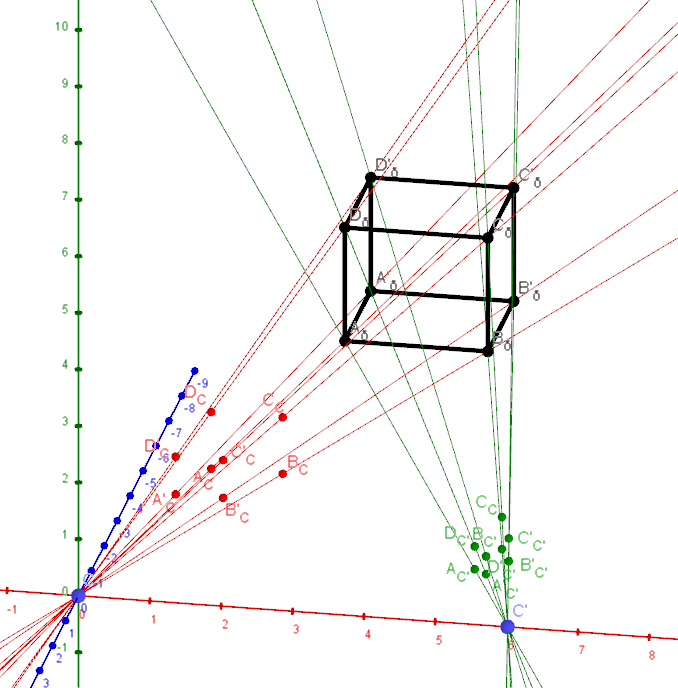
\includegraphics[width=\linewidth]{images/ScaleInvariance_1.png}
%	\caption{A really Awesome Image}
	\label{fig:awesome_image1}
	\endminipage\hfill
	\minipage{0.42\textwidth}
	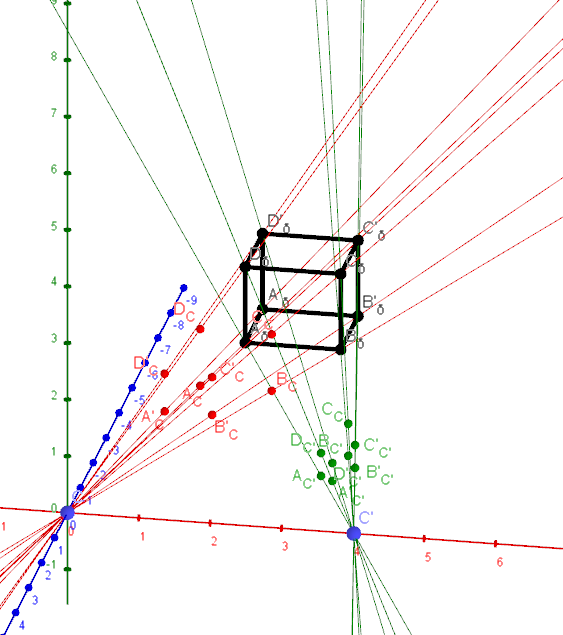
\includegraphics[width=\linewidth]{images/ScaleInvariance_2.png}
%	\caption{A really Awesome Image}
	\label{fig:awesome_image2}
	\endminipage\hfill
\end{figure}


\begin{minipage}{\linewidth}
	\centering
	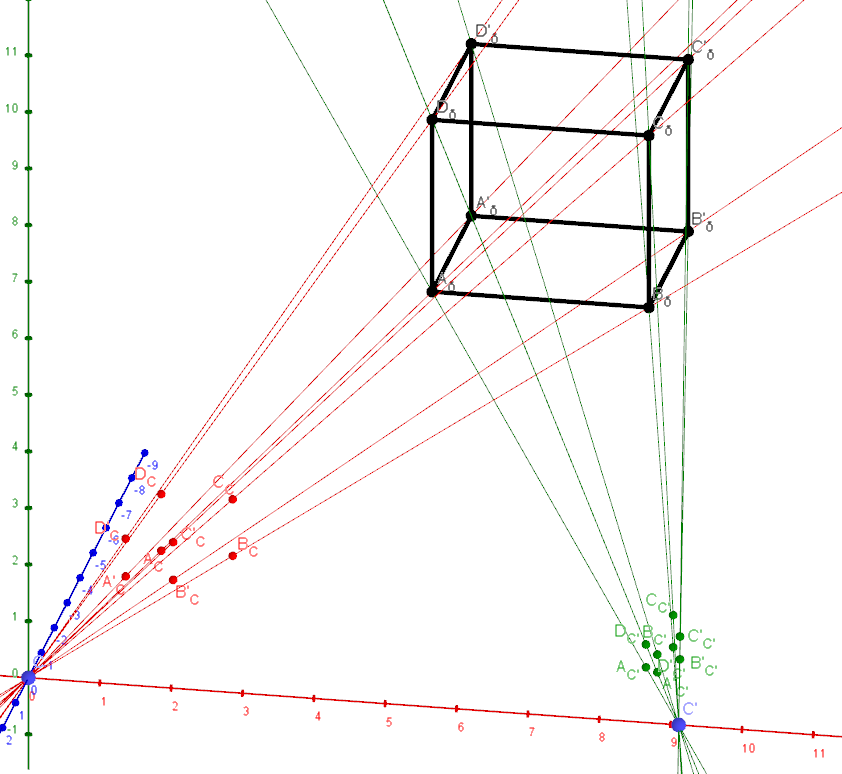
\includegraphics[width=0.42\linewidth]{images/ScaleInvariance_3.png}
	\captionof{figure}{Veranschaulichung der Skaleninvarianz und dessen Auswirkung auf die geometrische Form der Objekte} 
\end{minipage}\\ \\

\begin{figure}[!htb]
	\minipage{0.42\textwidth}
	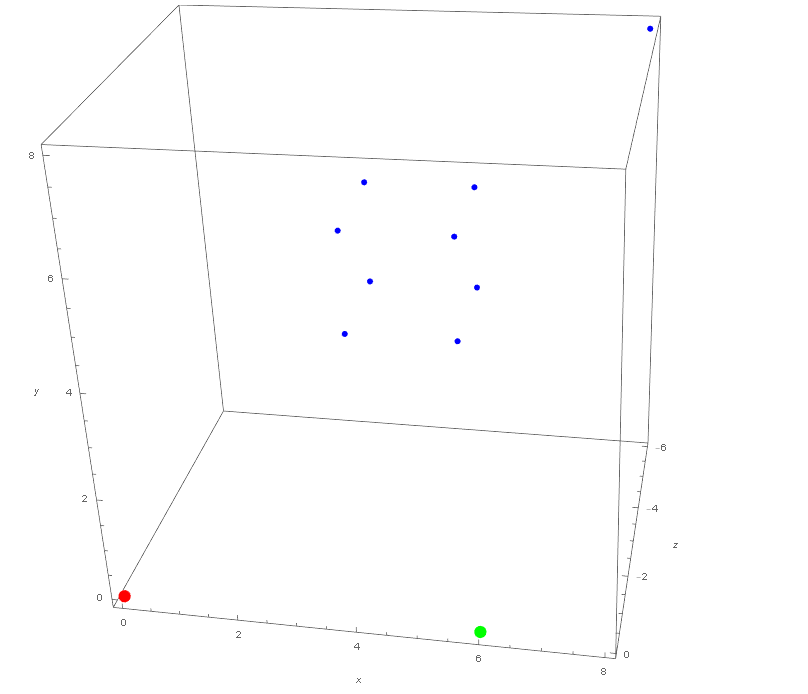
\includegraphics[width=\linewidth]{images/MinimalBeispiel_reconstructed.png}
	%	\caption{A really Awesome Image}
	\label{fig:awesome_image1}
	\endminipage\hfill
	\minipage{0.42\textwidth}
	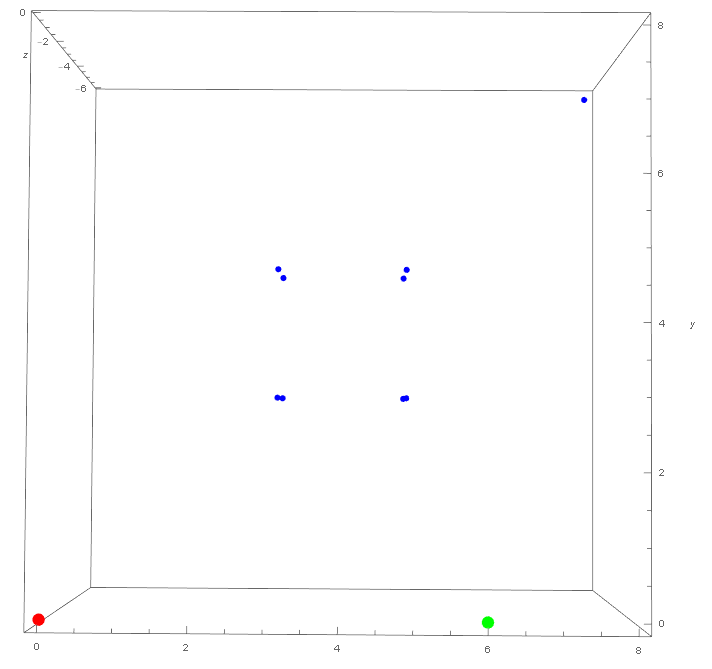
\includegraphics[width=\linewidth]{images/MinimalBeispiel_reconstructed_3.png}
	%	\caption{A really Awesome Image}
	\label{fig:awesome_image2}
	\endminipage\hfill
	\captionof{figure}{auf Originalgröße skalierte rekonstruierte Szene}
\end{figure}

\pagebreak
Abbildung 4.7 zeigt die Komplett rekonstruierte Szene des Minimalbeipiels, welche beweist, dass die beschriebenen Methoden für das Minimalbeispiel mit reinen Daten und auch bei Kameras mit unterschiedlichen Auflösungen, funktioniert hat. 

